\documentclass[twocolumn,amsmath,amssymb,pra]{revtex4-2}
\usepackage[utf8]{inputenc}
\usepackage{amsmath}
\usepackage{tabularx}
\usepackage{graphicx}
\graphicspath{ {figures/} }
\usepackage{siunitx}
\usepackage{hyperref}
\usepackage{float}
\newcommand{\eq}[1]{\begin{equation}#1\end{equation}}

\newcommand{\sub}[1]{_\textrm{#1}}


\begin{document}

\title{Physics 357-0: Fabry-P\'{e}rot Cavity Interferometry}

\author{Jun Sung and Thomas Douglas}

\date{25-Oct-2021}

\maketitle

\section{Introduction}
Optical cavities are devices which use mirrors in order to "trap" light to produce interference effects. In a Fabry-P\'{e}rot cavity, two parallel mirrors (which are usually not flat) are placed facing eachother in order to bounce light transmitted into the cavity between the two mirrors. These cavities show resonance effects due to the relationship between the frequency of incident light and the length of the cavity. These resonance effects can be quite complex and can display higher order modes. Optical cavities are extremely useful measurement tools, due to their high sensitivity. In this lab, we will observe resonance effects in the cavity and explain why and when we see them. We will explore other properties of Fabry-P\'{e}rot cavities and how these make them useful.

\subsection{A Brief Overview of Methods}
This lab consists of three main parts: 
\begin{itemize}
    \item[1] Observing the various spatial modes of the cavity
    \item[2] Calculating the Free Spectral Range of our cavity
    \item[3] Calculating the Finesse of our cavity
\end{itemize}
For the first part, we see how misaligning the cavity results in us observing various spatial modes of our cavity. As for how we actually view such modes, we use the CMOS camera along with the Thorlabs ThorCam software. 

For the second and third parts, we replace the CMOS camera with a transmission detector and add another reflection detector to our setup. Using these detectors (connected to an oscilloscope), we are able to view the transmitted/reflected resonant peaks from our laser, which in turn will allow for us to calculate the Free Spectral Range as well as the Finesse of our cavity. Furthermore, we will be using Python to analyze the data exported from the oscilloscope and calculate the wanted quantities.

\subsection{Applications}
Fabry-P\'{e}rot cavities are very useful due to the high degree of sensitivity of the cavity and high degree of control offered through methods such as Pound-Drever-Hall. These cavities are frequnelty used in creating optical wavemeters. The high degree of frequency sensitivity allows Fabry-P\'{e}rot inferometers to measure single atomic transitions and very small changes in atomic spectra due to the Zeeman effect. Cavities with extremely low energy loss (high quality factor) have even more applications. A notable example is the LIGO detector, which used km Michelson inferometers and Fabry-P\'{e}rot cavities to increase the effective path length and thus the sensitivity of the inferometer. This led to the successful detection of gravitational waves.

\section{Theory}

When light is incident upon an interface between two mediums, a portion of this light is reflected and a portion of this light is transmitted, described by the complex transmission and reflection coefficients $R$ and $T$ respectively, where we require $R^2 + T^2 = 1$ (the coefficients must be complex to account for a phase due to transmission or reflection). Such is the case when light is incident upon a mirror and when we place two mirrors a distance L apart we get the basic structure of a Fabry-P\'{e}rot cavity. To understand the basic principles of the cavity, we will simplify our analysis to light traveling one-dimension inside the cavity.

Generally, light interacting with the cavity is described by 
\eq{
\epsilon\sub{p,m,n}(z,t) = E\sub{p,m,n}e^{i\phi\sub{p,m,n}z - \omega{}t},
}
with indices $p$ corresponding to the incident, reflected, or transmitted portion of light incident upon mirror $m$ having completed $n$ trips through the cavity. When light is incident upon the first mirror, the portion of the light transmitted, with amplitude 
\eq{
    E\sub{i,2,0} = E\sub{t,1,0} = TE\sub{i,1,0}.
} 
will travel through the cavity and acquire a phase shift $ \delta = 2\pi{}L/\lambda$ each time it crosses, so the light incident upon the first mirror after one full trip is 
\eq{
    \epsilon\sub{i,1,1} = TRe^{i2\delta{}}\epsilon\sub{i,1,0}
}
The light incident upon the first mirror after crossing the cavity $n$ times is described by 
\eq{
    \epsilon{}\sub{i,1,n} = (Re^{i\delta{}})^{2(n-1)}\epsilon\sub{i,1,1} = TR^{-1}(Re^{i\delta{}})^{2n}\epsilon\sub{i,1,0}
}
Thus the light exiting the cavity on the side of the first mirror after $n$ trips is
\eq{
    \epsilon{}\sub{t,1,n} = \frac{(Re^{i\delta{}})^{2n}T^2}{R}\epsilon\sub{i,1,0}
}
This light will interfere with the light reflected off the first mirror $\epsilon\sub{r,1,0}$, such that
\eq{
    \epsilon{}_{\textrm{r,1},\infty} = \epsilon{}\sub{r,1,0} + \sum_{k = 1}^{\infty} \epsilon{}\sub{t,1,n} = \left(R - \frac{T^2}{R}\sum_{k = 1}^\infty(-Re^{i\delta{}})^{2k} \right)\epsilon\sub{i,1,0},
}
which can be simplified through the use of geometric series:
\eq{
    \epsilon{}_{\textrm{r,1}\infty} 
    = \left(R-\frac{T^2Re^{i2\delta{}}} {1-R^2e^{i2\delta{}}}\right)\epsilon\sub{i,1,0}
    = R\left(\frac{1 - (T^2+R^2)e^{i2\delta{}}} {1-R^2e^{i2\delta{}}}\right)\epsilon\sub{i,1,0},
}
or
\eq{
    \frac{\epsilon{}_{\textrm{r,1},\infty}}{\epsilon\sub{i,1,0}}  = R\left(\frac{1 - e^{i2\delta{}}} {1-R^2e^{i2\delta{}}}\right)
}
The steady-state intensity of the reflected light is given by the magnitude squared of this ratio
\eq{
    \frac{I\sub{r}}{I\sub{0}} =
    \left|\frac{E_{\textrm{r,1},\infty}}{E\sub{i,1,0}}\right|^2 = |R|^2\left(\frac{2-2\cos{2\delta{}}}{1+|R|^4-2|R|^2\cos{2\delta{}}}\right).
}

Likewise we can calculate
\eq{
    \epsilon{}_{\textrm{t,2},\infty} = \epsilon{}\sub{t,2,0} + \sum_{k = 1}^{\infty} \epsilon{}\sub{t,2,n} 
    = T^2e^{i\delta{}}\left(1 + \sum_{k = 1}^\infty (-Re^{i\delta{}})^{2k} \right)\epsilon\sub{i,1,0},
}
which simplifies to
\eq{
    \epsilon{}_{\textrm{t,2},\infty} 
    = \left(\frac{T^2e^{i\delta{}}} {1-R^2e^{i2\delta{}}}\right)\epsilon\sub{i,1,0}.
}
and for transmitted intensity, we get
\eq{ \label{I_t}
    \frac{I\sub{t}}{I\sub{0}} = \left|\frac{E_{\textrm{t,2},\infty}}{E\sub{i,1,0}}\right|^2
    = \frac{|T|^4} {1+|R|^4 - 2|R|^2\cos{(2\delta{}})}.
}
which can be simplified with the double angle identity
\eq{
    \frac{I\sub{t}}{I\sub{0}} = \frac{|T|^4} {(1 - |R|^2)^2 + 4|R|^2\sin^2{\delta{}}}
}
Thus the condition for peak transmission amplitude is
\eq{
    2\delta = \frac{4\pi{}L}{\lambda} = 2\pi{}m
}
or
\eq{ \label{peak}
    \frac{2L}{\lambda} = m
}
for any integer $m$. The intensity at peak transmission is
\eq{
    \frac{I\sub{t}^\textrm{max}}{I\sub{0}}
    = \left(\frac{|T|^4}{(1-|R|^2)^2}\right) = 1.
}


\subsection{Free Spectral Range (FSR)}

We can calculate the difference in frequency between resonant peaks satisfying Equation \ref{peak} by
\begin{align} \label{FSR}
    \Delta{}\nu\sub{FSR} &= \nu{}\sub{m+1} - \nu\sub{m}
    = c\left(\frac{1}{\lambda\sub{m+1}} - \frac{1}{\lambda\sub{m}}\right)
    = \frac{c}{2L},
\end{align}
and in a similar fashion, calculate the difference in cavity length between two peaks
\begin{align}
    \Delta{}L\sub{FSR} &= L\sub{m+1} - L\sub{m}\\
    &= \frac{\lambda}{2}.
\end{align}
The Finesse of a cavity is defined as 
\eq{
    F = \frac{\Delta{}\nu\sub{FSR}}{\Delta{}\nu\sub{FWHM}},
}
where $\Delta{}\nu\sub{FWHM}$ is defined as the linewidth of a frequency peak at half of its maximum intensity.
We can calculate the phase difference between when the intensity $I\sub{t} = 0.5 I\sub{t}^\textrm{max}$ using  Equation \ref{I_t}, when the denominator is twice as large as for peak intensity:
\eq{ 
    (1 - |R|^2)^2 + 4|R|^2\sin^2{\delta{}} = 2(1-|R|^2)
}
which implies
\eq{ 
    \sin^2{\delta{}} = \frac{(1 - |R|^2)^2}{4|R|^2}
}
thus
\eq{
    \delta{} = \pm \arcsin\left({\frac{1-|R|^2}{2|R|}}\right).
}
Since our mirrors have very high coefficients of reflectively,  $|R|^2 \approx 1$, thus the argument of the sine function is close to 0 and we can use a small angle approximation:
\eq{
   \delta{} \approx \pm \frac{1-|R|^2}{2|R|^2}
}
Thus the difference between half maximum frequencies before and after resonance is
\eq{
    \frac{2\pi{}L\Delta{}\nu\sub{FWHM}}{c} \approx 2\frac{1-|R|^2}{2|R|}
}
or 
\eq{ \Delta{}\nu\sub{FWHM} \approx \frac{c}{\pi{}L}\frac{1-|R|^2}{2|R|}.
}
Now we can use Equation \ref{FSR} to give the cavity finesse:
\eq{ 
    F \approx \frac{\pi{}|R|}{1-|R|^2}.
}

\subsection{The Quality Factor: Q}
Our analysis thus far has assumed an ideal cavity, with no light intensity loss due to scattering. For light contained inside the cavity, transmission out of the cavity and random result in a loss of energy during each cycle. The loss of energy due to transmission is described by the transmittance of the mirrors
\eq{ 
    \frac{I}{I_c} = T^2
}
The loss of energy due to scattering is described by 
\eq{ 
    \frac{I}{I_c} = e^{-\alpha L}
}
where $I_c$ is the intensity of light inside the cavity. Taking both of these into account, we can estimate the energy lost from the cavity per cycle (the period of the light) by
\eq{
    \epsilon\sub{lost} = \frac{2\lambda{} T^2 I_c}{c}e^{-\alpha\lambda}
}
where we have replaced $L$ with $\lambda$ since the light moves exactly one wavelength per cycle. Since the internal intensity of light $I_c$ is describes the power per unit area, the internal intensity of light is given by multiplying by twice the length of the cavity ($2L$). Dividing by the wavelength gives the total internal intensity per wavelength, and we must divide by the frequency to get the internal intensity per cycle. This gives
\eq{
     \epsilon\sub{stored} = \frac{2L I_c}{c}.
}
Thus the quality factor is given by 
\eq{ 
    Q = \frac{\epsilon\sub{stored}}{\epsilon\sub{lost}} \approx \frac{L}{(1-R^2)\lambda}
}
where we have used that $T^2 = 1 - R^2$.


\subsection{The Laser Diode}
For this experiment, we use a laser diode to create our laser. Such a device which uses the same operating principle as a Light-Emitting Diode (LED). Light is produced at the boundary of a p-type (more electrons present) and n-type (more holes present) semiconductor due to a voltage applied across the junction. Semiconductor p-n junctions create depletion layers between the two materials due to their differing charge densities. When a bias is applied to this junction, electrons and holes flow between the two regions, and across this depletion layer. As charges move between the materials, recombination mechanisms allow for carrier annihilation and the emission of photons at energies around the semiconductor bandgap (although the frequency of photons leaving the laser is controlled by the internal Fabry-Perot cavity). 

We control the frequency of the laser through the current passing through the diode. An increase in current results in an increase in electron hole pairs inside the diode, which results in a higher intensity, but also reduces the effective length of the internal cavity of the diode, changing the frequency of light leaving the laser. The diode laser is very sensitive, so small changes in temperature can change the frequency of the laser. For this reason we use a temperature controlled casing to maintain a consistent temperature within the diode laser.




\section{Apparatus}

\subsection{Apparatus Design}
The design of our apparatus has the purpose of preparing the laser such that it enters the cavity in a controlled and desired way. We first use a diffraction grating to filter the frequencies of the laser, then we use a Faraday lens to limit the intensity of light reflected into the laser. This protects the laser from damage and allows a longer lifetime. Next, the beams is directed through a fiber-optic cable, which isolates a  transverse mode of the laser, as other modes are not of interest for this lab. The beam is then passed through a lens, which focuses the beam. Next the beam passes through the EOM, which allows us to modulate the phase of the beam, as is used in PDH locking. The extent of our data did not utilize this phase modulation. Next the beam passes through a 50:50 beam splitter, which allows us to measure the reflected intensity of the beam as it returns from the cavity. Next the laser enters the cavity. We can adjust the beam splitter and one mirror to control the incident alignment of the beam on the cavity. The adjustment of these two elements is what allowed us to view different TEM modes. A CMOS camera is used to observe the intensity pattern of the transmitted light and a photodetector was used to monitor the intensity of reflected light (after passing through the beam splitter). The cavity is connected to a piezoelectric controller, which allows us to use an AC function generator to periodically modulate the cavity length. This was used to measure throughout the lab to observe resonance phenomena, because periodic modulation of the laser frequency is difficult to do due to the age of the laser and precision of equipment.


\subsection{TEM Observation Apparatus}
\begin{figure}[htbp]
    \centering
    \includegraphics[ width = 0.9 \linewidth ]{apparatus-1.jpg}
    \caption{The apparatus used to view the spatial modes of the cavity}
    \label{fig:app_1}
\end{figure}



The setup that we used to view the spatial modes of our cavity can be seen in Figure \ref{fig:app_1}.
It should be noted that most of the apparatus was aligned for us before we started the lab; in particular, the alignment of the laser such that it passes through the fiber mode cleaner and EOM was done by Prof. Watkins and Prof. Kovachy. Furthermore, the cavity mirrors (both front and rear) were already adjusted for us as well. Our contribution to the alignment process came in the form of adjusting the 50:50 BS as well as the mirror directly above it. What adjusting these allowed for us to do was to "misalign" the cavity without adjusting the cavity mirrors -- that is, we were able to adjust the direction in which the laser would be incident on the front mirror to emulate the cavity being misaligned. It is from adjusting the 50:50 BS and the mirror directly above it that we were able to observe the different spatial modes of the cavity. What is not shown in Figure \ref{fig:app_1} is the Thorlabs ThorCam software we used to view the input going into the CMOS camera.


\subsection{Reflection and Transmission Measurement Apparatus}
\begin{figure}[htbp]
    \centering
    \includegraphics[ width = 0.9 \linewidth ]{apparatus-2.jpg}
    \caption{The apparatus used to view the transmission and reflection peaks from our laser and cavity}
    \label{fig:app_2}
\end{figure}
The setup that we used to calculate the FSR and Finesse of our cavity can be seen in Figure \ref{fig:app_2}. The only difference in this setup when compared to the first is that the CMOS camera is replaced with a transmission detector, and we have also added a reflection detector as well. It should be noted that our original reflection detector went missing, and neither us nor Prof. Watkins and Prof. Kovachy were able to locate it during our time doing the lab. In fact, the reflection detector shown in Figure \ref{fig:app_2} is just another transmission detector (albeit, an older model of our first transmission detector). Thus, we were not able to measure the Finesse of the cavity in the way that the lab guide intended. This issue we faced will be discussed more in detail in the data collection section of our lab report. Although it isn't labelled in Figure \ref{fig:app_2}, we used an oscilloscope to view the output of our transmission detector.

Table \ref{tab:parts} lists all the main components in both of the setups (as well as their function) that we used throughout this lab. The Reflection Power Detector is one of the elements of our equipment which was not available to use in completing this lab. As a result, we had difficulty in obtaining accurate measurements of the cavity finesse, which we will discuss later.
\begin{table}[htbp]
\centering
\caption{Apparatus Parts} 
\label{tab:parts}
\begin{tabular}{|p{0.22\linewidth}|p{0.5\linewidth}|p{0.2\linewidth}|}
 \hline
 \textbf{Name}
 &
 \textbf{Function}
 &
 \textbf{Part Number}
 \\
 \hline
 EOM
 &
 To modulate the laser beam. This will allow for us to find both the FSR and Finesse of the cavity.
 &
 EO-PM-R-20-C1
 \\
 \hline
 50/50 Beam Splitter
 &
 Splits our laser beam half-half. This will allow for us to observe different spatial modes as well as help with finding the FSR and Finesse of the cavity.
 &
 BSW10
 \\
 \hline
 Front Mirror
 &
 Cavity front mirror. It is a flat mirror ($R=\infty$) with reflectivity of about 99\%
 &
 BB1-E03
 \\
 \hline 
 Rear Mirror 
 &
 Cavity rear mirror. It is a concave mirror ($R = 3 \si{m}$) with reflectivity of about 99.9\%
 &
 TLM1-780-0-1025-3.00C
 \\
 \hline 
 Transmission Power Detector
 &
 To measure the transmission power. We should note that this detector has a high gain, but low response time ($\tau \sim 100 \si{\mu s}$).
 &
 PDA36A2
 \\
 \hline 
 Reflection Power Detector
 &
 To measure the reflected power. Note that this detector has a low gain, but fast response time ($\tau< 10 \si{n s}$).
 &
 PDA10A
 \\
 \hline 
 CMOS Camera 
 &
 To observe the special mode of the Fabry-P\'{e}rot cavity. This camera also helps us align the cavity in the beginning.
 &
 DCC1545M
 \\
 \hline
\end{tabular}
\end{table}
Furthermore, Figure \ref{fig:app_3} shows the Laser Diode Controller, Function Generator, and Piezo controller.
\begin{figure}[htbp]
    \centering
    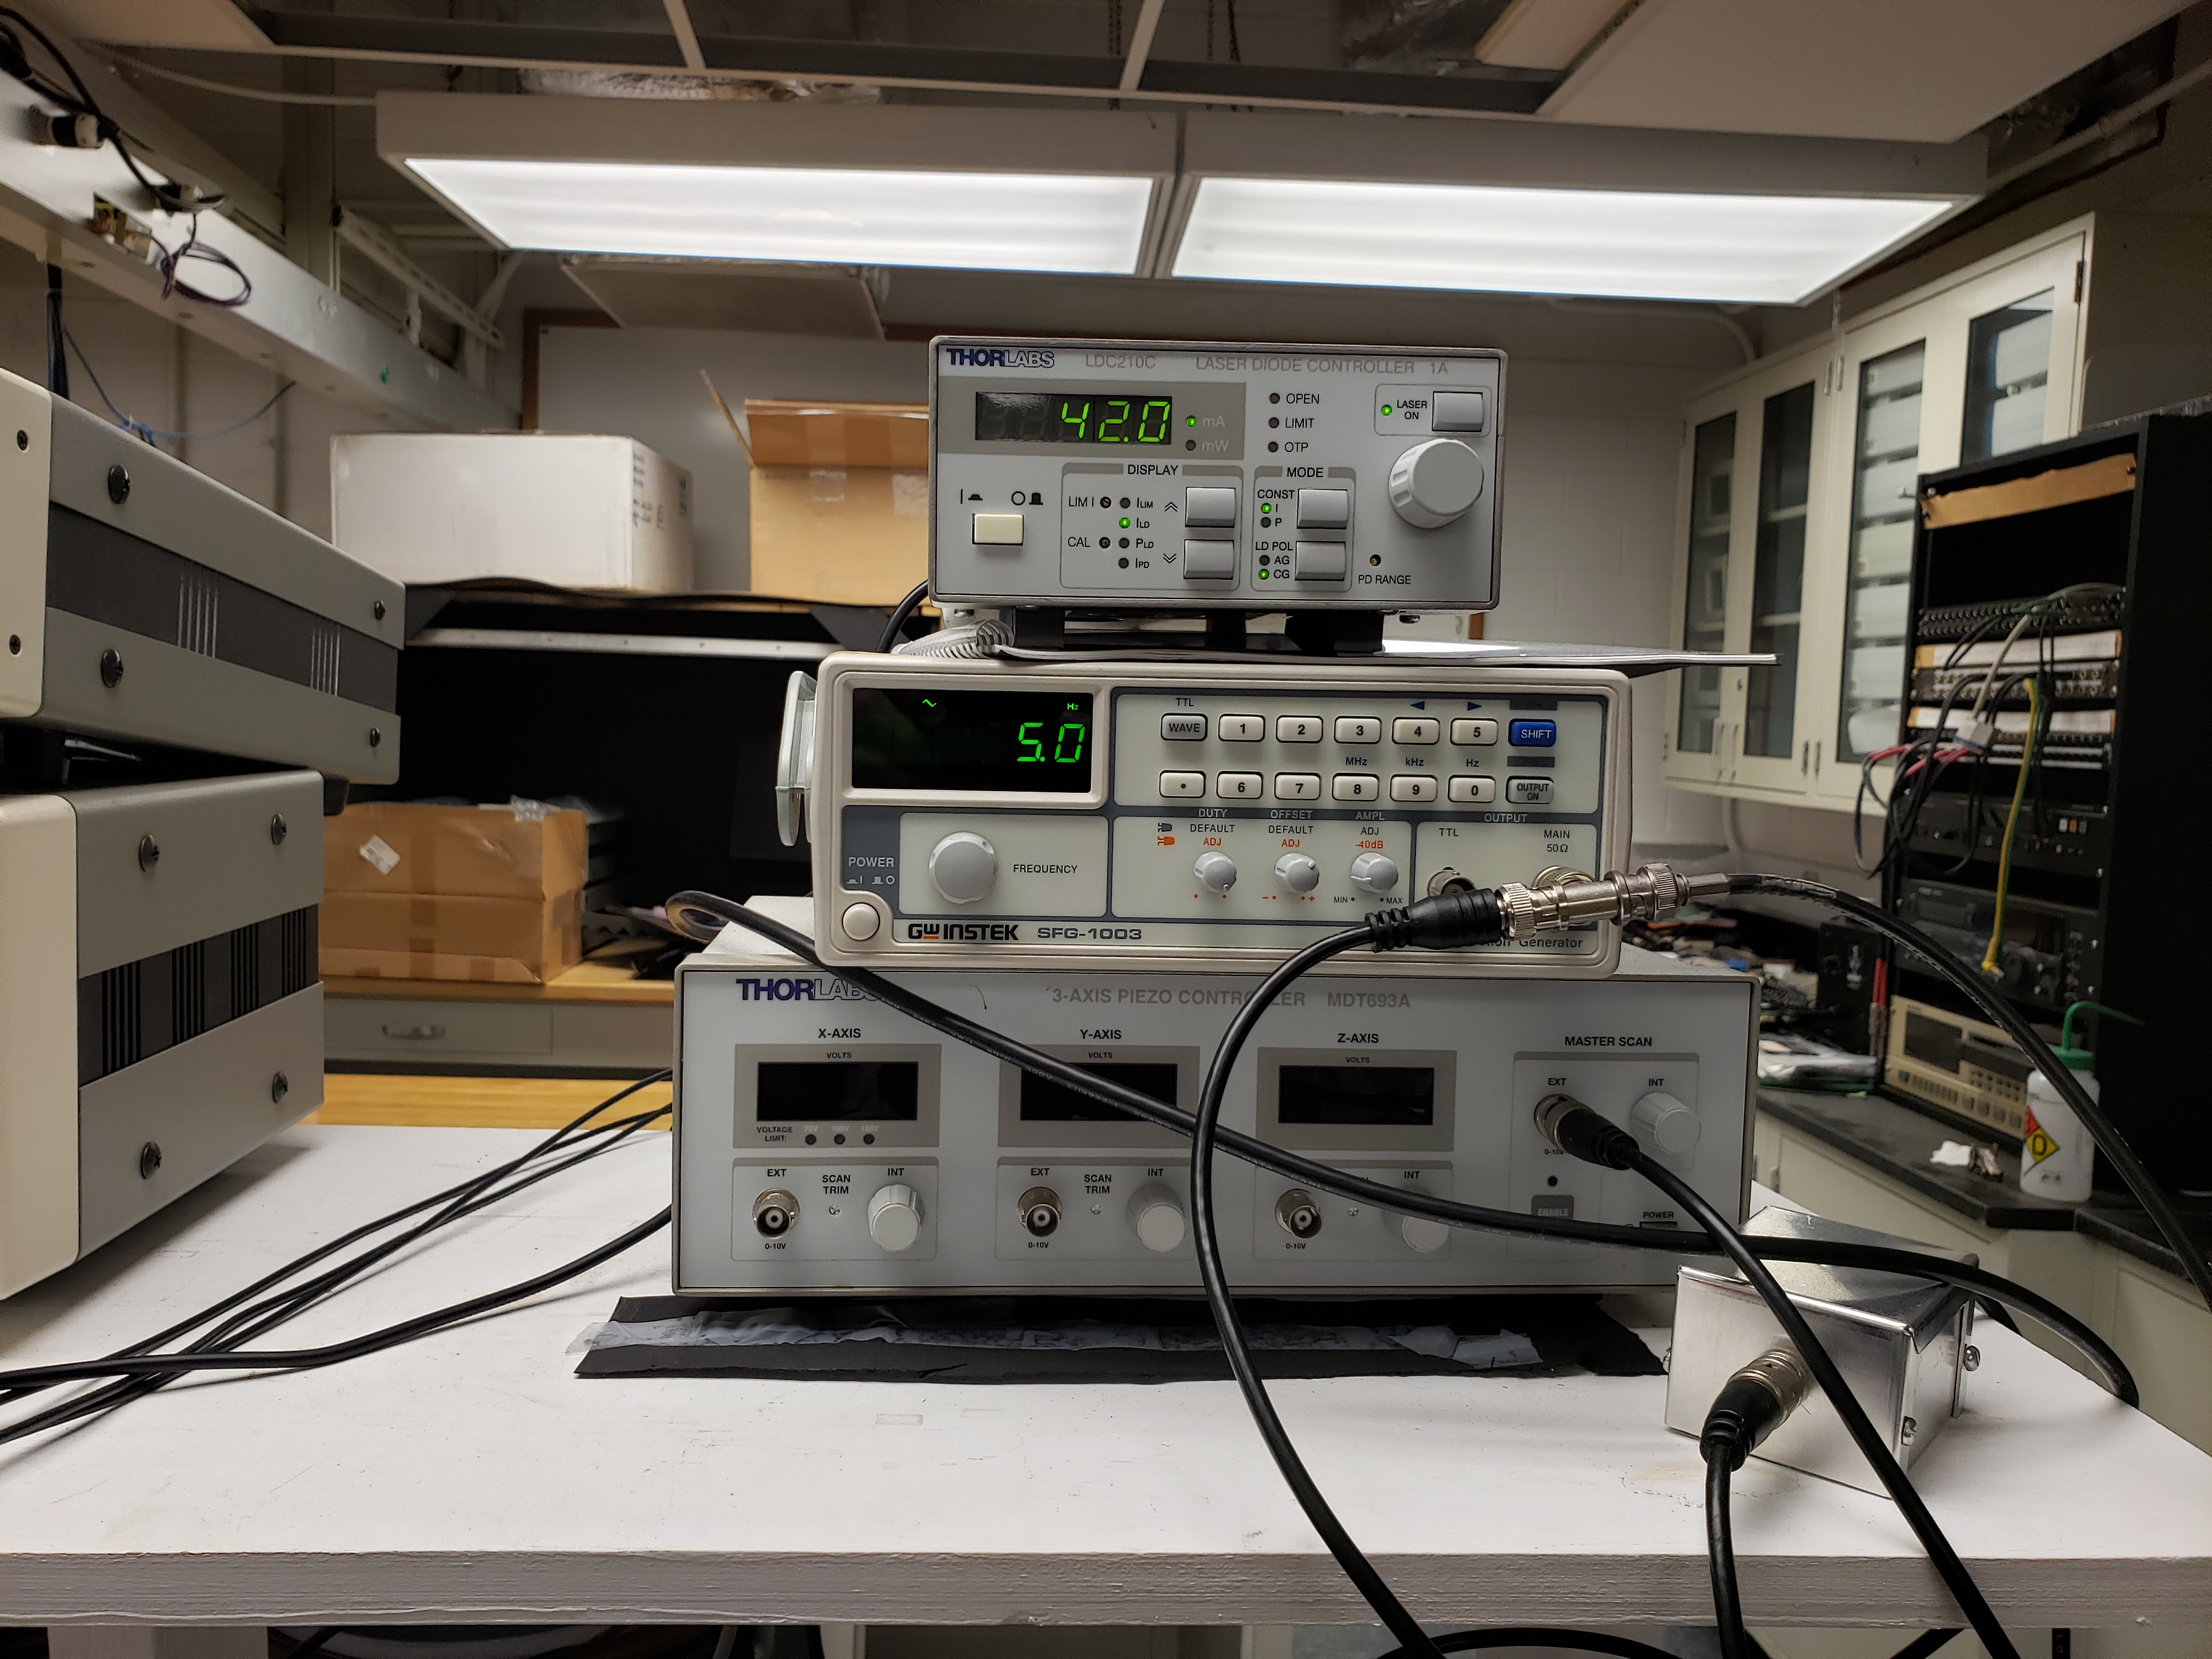
\includegraphics[ width = 0.9 \linewidth ]{apparatus-3.jpg}
    \caption{The Laser Diode Controller, Function Generator, and Piezo Controller used for this lab}
    \label{fig:app_3}
\end{figure}
The Laser Diode Controller allows for us to adjust the current of our laser, and we shall discuss more about the Function Generator and Piezo Controller in the data collection section of this lab report.

\section{Measurements and Data Analysis}
\subsection{Data Collection}
\subsubsection{Looking at Different Spatial Modes}
As discussed briefly in the apparatus section of this lab manual, we adjust the 50:50 BS along with the mirror directly above it to emulate the misaligning of the cavity. To see just how badly the cavity is misaligned, we look at the transmission of the cavity via the CMOS camera and Thorlabs ThorCam software. We should expect to see a bright, round cavity output if we aligned everything correctly (as seen in the top left picture in Figure \ref{fig:tem_modes}). However, if the cavity is misaligned in any way, then the outputs we see differ from a bright, round spot; in fact, the different outputs correspond to different spatial modes of our cavity which can be described with Hermite Gaussian functions. The different modes can be identified by the number of resonance peaks we observe. These appear as bright spots on our camera, and modes of different orders (with different numbers of peaks) can be observed in the horizontal and vertical direction simultaneously. We began by observing the bright, round output to correspond to the TEM00 mode, and we played around with adjusting the 50:50 BS and mirror to obtain as many other TEM modes as we could.

\subsubsection{Free Spectral Range}
As discussed in the introduction of our lab report, the FSR refers to the frequency between resonant peaks. Such a quantity was derived upon the assumption that our cavity length remains fixed while our laser's wavelength/frequency is allowed to vary. However, in our case, the lab manual had us keep the laser's wavelength/frequency to be fixed while our cavity length varies. The way that we varied the cavity length was via the piezo crystal; by applying a voltage across it, we were able to change the length of the crystal. From discussing with Prof. Watkins, we determined how to calculate the change in crystal length per voltage by multiplying the piezo electric coefficient with the length of our piezo crystal. The values that Prof. Watkins provided for both of these quantities resulted in us getting $60 \ \si{nm}$ per $V$. 

To utilize this information, we need to figure out how much the piezo crystal changes lengthwise between resonant peaks so that we can find the cavity length between these resonant peaks. We started by getting our cavity aligned such that the spatial mode being transmitted through was the TEM00 mode. Once this was in place, we changed our setup to what is shown in Figure \ref{fig:app_2}. For this part of the lab, we only need to display the output of the transmission detector as well as the function generator (which we set to be a triangular wave pattern). The reason for displaying the function generator output is because we also have the piezo controller connected to the function generator -- thus, we can calculate the change in voltage between two resonant peaks, which then allows for us to calculate the change in length of the piezo crystal between resonant peaks using the result that our piezo crystal's length changes $60 \ \si{nm}$ per $V$. One important note that we need to mention is that our piezo device multiplies the voltage by 10, meaning that if we see $2 V$ in the oscilloscope, this corresponds to $20 V$ being applies to the crystal. Figure \ref{fig:eg_data_fsr} shows an example of the type of data we took during this part of the lab. 
\begin{figure}[htbp]
    \centering
    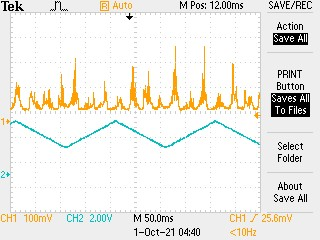
\includegraphics[ width = 0.9\linewidth ]{example_data_fsr.jpg}
    \caption{An example for the type of data we took when calculating the change in length between resonant peaks}
    \label{fig:eg_data_fsr}
\end{figure}

\subsubsection{Finesse}
In the introduction, we noted that the Finesse of a cavity is defined as the ratio of the FSR to the linewidth of a frequency peak at half of its maximum intensity. However, this quantity has a more physical meaning; namely, it describes the amount of times light bounces inside a cavity before it escapes. Thus, if the cavity is very large, then it would take the light a long time to escape from the cavity. Therefore, we can measure how long the accumulated light takes to escape the cavity, which we can then convert to the Finesse of our cavity. 

We use the same setup as in Figure \ref{fig:app_2} for this part of the lab. Notice that our reflection power detector needs to have a very fast response time ($\tau < 10 \ \si{ns}$), otherwise we won't be able to measure the Finesse. By taking the reflection light and triggering the dip of the reflection power, we should see a feature similar to what is shown in Figure \ref{fig:eg_finesse}.
\begin{figure}[htbp]
    \centering
    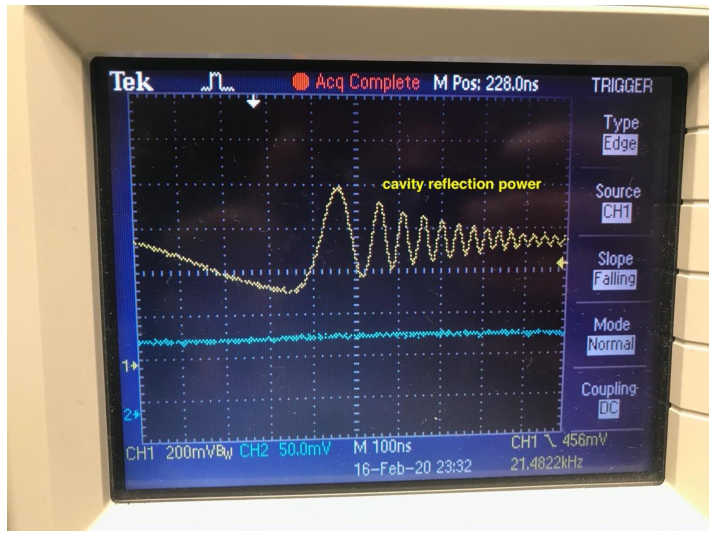
\includegraphics[ width = 0.8 \linewidth ]{finesse_eg.PNG}
    \caption{The expected feature when measuring for the Finesse of our cavity}
    \label{fig:eg_finesse}
\end{figure}
We can then extract this feature from the oscilloscope and fit the envelop of this oscillating decay, which is given by 
\begin{equation}
    \exp \left( - \frac{t}{2 \tau_{\mathrm{FP}}} \right)
    \quad 
    \mathrm{where}
    \quad 
    \tau_{\mathrm{FP}} = \frac{F L}{2 \pi c}
\end{equation}
where $F$ is the Finesse of our cavity and $L$ is the distance between the two mirrors. It is from this fit that we are able to measure the Finesse.

In our situation, though, we were not able to measure the Finnese this way since our reflection power detector went missing. The only detectors that we had were transmission detectors (which has a much larger time constant), which were insufficient when it came to seeing the feature shown in Figure \ref{fig:eg_finesse}. Thus, we instead worked with finding the ratio of the FSR to the linewidth of a frequency peak at half of its maximum intensity.

\subsection{Data Analysis}
\subsubsection{Free Spectral Range}
To calculate the change in length of the piezo crystal between resonant peaks, we used python -- namely, the \texttt{pandas} package. With this package, we were able to locate the times at which the resonant peaks occurred; we started off by extracting the csv data (from the oscilloscope) using the \texttt{pandas} package. The extracted data would be in contained in a \texttt{pandas.DataFrame} object, which would then allow for us to find the resonant peaks via the \texttt{pandas.DataFrame.iloc} method. Figure \ref{fig:eg_peaks}
\begin{figure}[htbp]
    \centering
    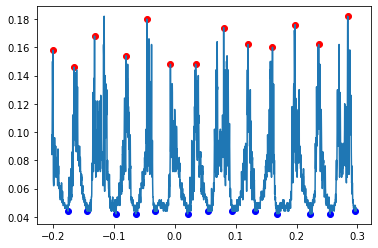
\includegraphics[ width = 0.8 \linewidth ]{peak_transmission.png}
    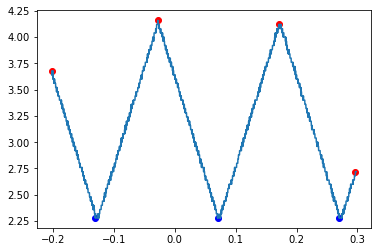
\includegraphics[ width = 0.8 \linewidth ]{peak_function_generator.png}
    \caption{The top picture shows the detected peaks of our resonant peaks, and the bottom picture shows the detected peaks of the output from the function generator}
    \label{fig:eg_peaks}
\end{figure}
With the peaks known, we were then able to utilize the \texttt{pandas.DataFrame.loc} method to find the corresponding times for each of the resonant peaks.
Once we knew these times, we could then find the corresponding voltages from the function generator using the same method just mentioned. We then calculated the change in voltages from the function generator between resonant peaks (making sure that there is not a peak these change in voltages do not take place), which we further converted to how much the piezo crystal's length changes using the conversion factor of $600 \ \si{nm}$ per $V$. We repeated this procedure for each capture we took from the oscilloscope.

\subsubsection{Finesse}
As noted in the data collection portion of this lab report, we had to resort to finding the ratio of the FSR to the linewidth of a frequency peak at half of its maximum intensity. To do so, we first needed to find the FSR; this required us to know the length of the cavity, which we found to be 
\begin{equation}
    L = 9.4 \pm 0.2 \ \si{cm}
\end{equation}
The uncertainty in this measurement is due to the use of imprecise measurement equipment and difficulty discerning the edge of the mirrors within the holders. Using Equation \ref{FSR}, we can calculate $\Delta \nu{}\sub{FSR} = 1.596 \ \si{GHz}\pm 33.95 \ \si{MHz}$. This uncertainty is propagated from the uncertainty in L, assuming the uncertainty in $c$ is negligible (a valid assumption considering the large uncertainty of our measurement). All we needed to do was to find the linewidth of a frequency peak at half of its maximum intensity, and then we could calculate the cavity Finesse. However, we came across many issues, which will be discussed in the results section of this lab report.

\subsection{Results}
\subsubsection{The Different Spatial Modes}
After playing around with the alignment of the 50:50 BS and the mirror directly above it, Figure \ref{fig:tem_modes} shows all the TEM modes we were able to observe. The 00, 01, and 10 modes were relatively easy to observe, however the other two required precise changes in the beam alignment in order to get a clear view of them. We were able to change the profile of the resonant peaks while maintaining the same mode by using a "walking" alignment method, where the vertical and horizontal axes of both alignment elements were adjusted in tandem, such that the compensated to preserve a clear view of the resonant mode.
\begin{figure}[htbp]
    \centering
    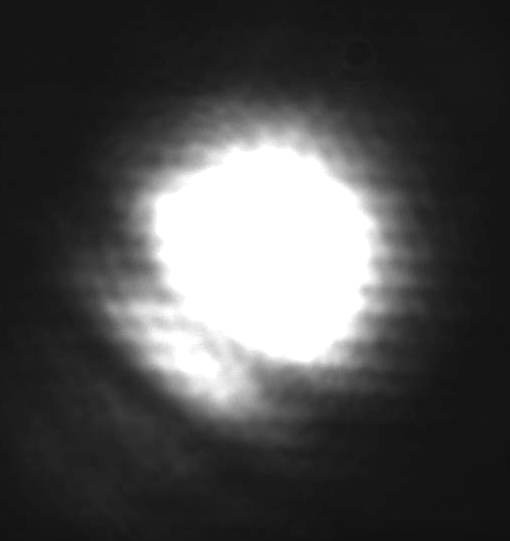
\includegraphics[ width = 0.45 \linewidth ]{TEM00.PNG}
    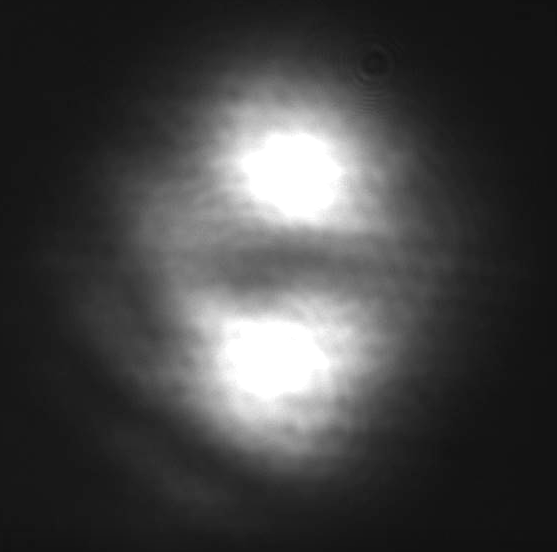
\includegraphics[ width = 0.45 \linewidth ]{TEM01.PNG}
    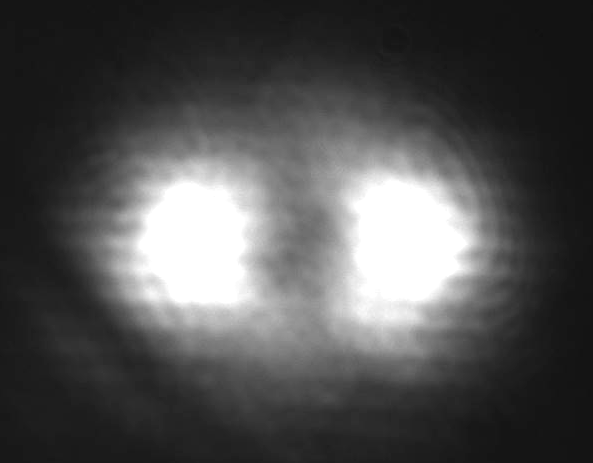
\includegraphics[ width = 0.45 \linewidth ]{TEM10.PNG}
    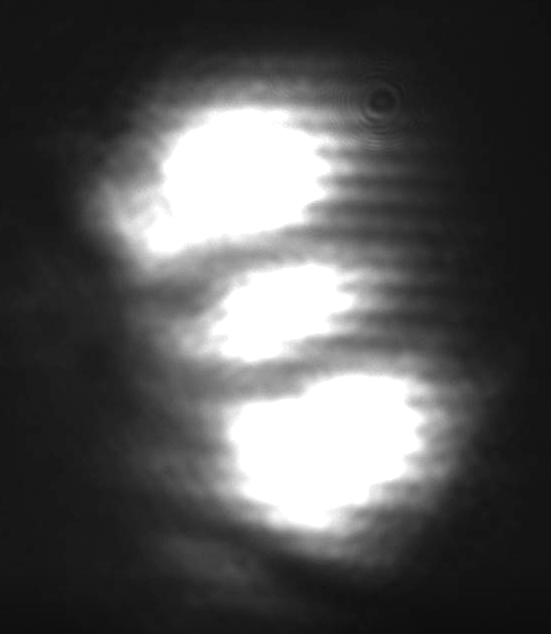
\includegraphics[ width = 0.45 \linewidth ]{TEM02.PNG}
    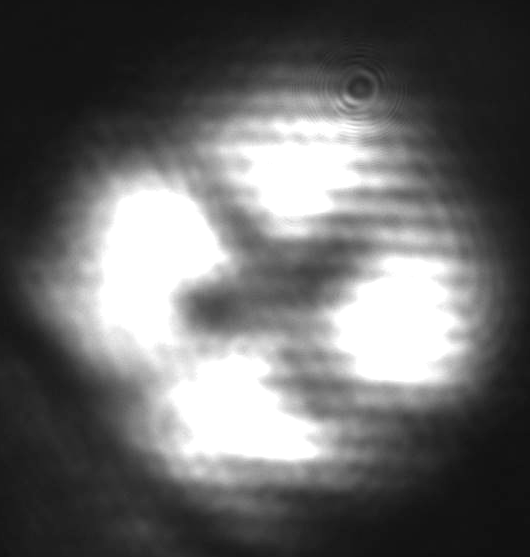
\includegraphics[ width = 0.45 \linewidth ]{TEM11.PNG}
    \caption{The top left, top right, middle left, middle right, and bottom pictures correspond to the TEM00, TEM01, TEM10, TEM02, TEM11 modes, respectively.}
    \label{fig:tem_modes}
\end{figure}

\subsubsection{Free Spectral Range}
Using the methodology described in the data analysis portion of this lab report, we found the following values for the change in cavity length between resonant peaks
\begin{table}[htbp]
\centering
\caption{The Calculated $\Delta L$} 
\label{tab:fsr}
\begin{tabular}{|p{0.22\linewidth}|p{0.5\linewidth}|p{0.25\linewidth}|}
\hline
\textbf{Trial}
&
\textbf{$\Delta L$ Mean (nm)}
&
\textbf{$\Delta L$ Std (nm)}
\\
\hline
1
&
318.0
&
118.6
\\
\hline
2
&
364.0
&
66.3
\\
\hline
3
&
368.0
&
64.0
\\
\hline 
4
&
323.2
&
122.0
\\
\hline 
5
&
356.0
&
36.4
\\
\hline 
6
&
307.2
&
140.0
\\
\hline 
7
&
423.0
&
43.2
\\
\hline
8
&
428.6
&
32.5
\\
\hline
\textbf{Total}
&
379.2
&
7.4
\\
\hline
\end{tabular}
\end{table}

\subsubsection{Finesse}
As noted earlier, all that we needed to do was to find the linewidth of a frequency peak at half of its maximum intensity. 
To do so, we used the \texttt{pandas} package again to get to this value. We used the same extracted data (all contained in a \texttt{pandas.DataFrame} object) that we collected for the FSR. We then used the \texttt{pandas.DataFrame.loc} method to find the corresponding times at which these half peaks occurred.
However, locating the times where the half peaks occurred proved to be difficult since the discrete time spacing from the oscilloscope was not fine enough; that is, there were rarely any times in our data where half peaks occurred. The way that we worked around this was to interpolate the data so that we can at least estimate at which times the half peaks would occur. We need to mention that interpolating the data was a last-ditch effort since we were not guaranteed that the interpolated times were correct. Furthermore, we found out in the end why the lab manual had us find the cavity length difference between peaks (rather than FSR) and the Finesse the way that it did -- there was no way for us to convert the data that we got into the corresponding frequency. If there were a way, then we could have just measured the necessary times for each parts of our experiment, and then convert all these times into frequency to get our desired results.

\section{Discussion}
Before we move onto how consistent our results from this lab was when compared to the theory, we start off by noting a couple remarks:
\begin{itemize}
    \item The lab manual had us measure the cavity length difference in place of the Free Spectral Range of the cavity.
    \item Our reflection power detector was unavailable, which meant that we were forced to use a detector with response time below that which is ideal to measure cavity finesse.
\end{itemize}
To expand on the second remark, we should note that we spent a few lab days trying to measure the Finesse using another transmission detector (which had a response time below what we needed). Even after all the time we spent on trying to make the detector work, we were still unable to produce the feature we wanted (as shown in Figure \ref{fig:eg_finesse}). Thus, we were not able to obtain any measured value for our Finesse.

\subsection{Discussion of Results}
We were able to clearly observe a number of resonant modes of the cavity. These show the Hermite Gaussian functions that give rise to spatially periodic resonant peaks in the transmission intensity of the beam. The use of a Fabry-P\'{e}rot as an inferometer is usually based upon observation of the first TEM mode, since this is all that is needed and gives the highest sensitivity frequency measurements. However, studying the properties of these cavities helps us understand how they work and the emergent phenomena from periodic interference of light waves. Some of these modes are shown in Figure \ref{fig:hermite_gaussian}.
\begin{figure}
    \centering
    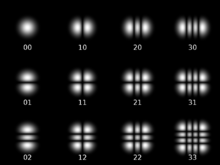
\includegraphics{Hermite-gaussian.png}
    \caption{The first twelve Hermite Gaussian Modes}
    \label{fig:hermite_gaussian}
\end{figure}
We were also able to observe the periodic resonance of the cavity as the length is varied, analogous to the peaks which are periodic in frequency. The FSR of a cavity is an important metric, which is of great interest to those using Fabry-P\'{e}rot cavities in measurement, since it determines to what range you can determine the frequency of any given incoming resonant signal.

Our result for $\Delta L$ was within $2 \sigma$ of what we expected (that being $\frac{\lambda}{2} = 392.5$), which makes our measured result consistent with what we would expect to observe.



We attempted to measure the Finesse of the cavity by observing the decay rate of the reflected intensity following a sharp peak. Unfortunately, we were unable to observe this decaying behavior due to the low response time of our detector and the noise of our laser frequency. 

\subsection{Sources of Error}

One possible source of error while we did our experiments could be from the laser itself. During our experiments, we found it difficult to keep the laser steady in general -- not just in the resonant modes; it was a common observation that the laser fluctuated greatly, such that the laser would move entirely off resonance. In turn, we think that this also means that the frequency of our laser was not as stable as we would have wanted, which in turn would have affected the values for $\Delta L$ that we got when we measured the cavity length differences between resonant peaks; This results in inconsistent periodicity for the resonant length measurements. We also measured the length of the cavity by hand, with measurement tools that are very imprecise compared to the sensitivity of the cavity. This means there is a large uncertainty in our free spectral range calculation.

Another source of error that we need to address would be the outside interference. To expand on this, our detectors required for us to be in the dark, and this in turn made it difficult for the other people in the room to see their experiment. Thus, there were a lot of external light (either from other people's phone flashlights, or from the light from the hallway) that resulted in artificial peaks to show up on the oscilloscope. However, we think that this was not much of an issue since we waited these external interferences out -- meaning that they did not have much of an influence (if at all) to our calculations.

Finally, one other possible source of error could have come from the peak-finding program used for this lab. While finding the peaks, the program found potential peak times -- some of which were incredibly close to each other. To account for these incredibly close values, we chose to keep one of such values and removed the rest since the difference in time between these values seemed negligible. We think that this is most likely fine for a single peak, but when there are many more peaks for which this problem occurs, these errors could add up to something non-negligible. 
The most notable effect that this error would have on our results would be the results we calculated for $\Delta L$ -- that is, there could be some slight errors to the values that we calculated using the program. However, we think that this error would be considerably less than if we were to do all this by hand, and the amount of times that we had peak times incredible close to each other were few and far between.

\section{Conclusion}
We have discussed the theory of Fabry-P\'{e}rot cavities, including deriving quantities of interest with respect to the behavior of the cavity. We have discussed how the properties of these cavities can be utilized to create very accurate  inferometers. We have also observed the phenomena predicted from the theories we discussed, including the resonant modes of the cavity and the periodic transmission intensity peaks. We used the values that we measured to characterize the length sensitivity of the cavity and made an estimate of the frequency sensitivity. We have attempted to measure the cavity finesse, although our results were impeded by equipment limitations.
Apart from the obvious ways that we could have improved the experiment (these being having a more stable laser and a reflection power detector), one possible improvement we could implement next time would be to build an encasing around the setup to reduce outside noise/interference; this would allow for our detectors to more accurately pick up the transmitted/reflected light, which in turn would result in more accurate measurements for all the parts of this lab.
Another possible improvement would be to better account for error in both the peak-finding and width-finding programs. As noted in the sources of error part of this lab report, we could have made better efforts to account for the very close peak times that we removed. This in turn would have made our calculation more accurate in the future if we ever wanted to repeat the experiment/calculations made more times.

\section{Figure References}
Figure \ref{fig:eg_finesse} can be found in the Cavity Lab Guide, and Figure \ref{fig:hermite_gaussian} can be found on \cite{wiki:HG}.

\bibliographystyle{unsrt}
\bibliography{References}

\end{document}